\documentclass[../main.tex]{subfiles}
\begin{document}
\chapter{Estado del Arte}
\section{Materiales Magnéticos y sus Propiedades}
Debido a que se busca caracterizar las propiedades magnéticas de los materiales de interés en esta tesis, es necesario puntualizar algunas características de interés.
\subsection{Magnetización}
La magnetización (M) de un volumen determinado se define como la suma de los momentos magnéticos contenidos dentro de éste. Representa la dirección y fuerza del campo magnético macroscópico resultante.

Ésta puede ser inducida por un campo magnético externo (H), como se explicará es el caso de los materiales para y diamagnéticos, o ser producto de un orden intrínseco de los átomos que forman el material, como es el caso de los ferro, antiferro y ferrimagnéticos. Sin embargo, incluso en este último caso, el campo magnético externo sigue teniendo efecto en la magnetización.

A excepción únicamente del diamagnetismo, los materiales magnéticos dependen de la alineación de sus momentos de espín, lo cual se traduce en una dependencia de la magnetización y la susceptibilidad magnética en la temperatura, debido a que el ordenamiento de los momentos se ve afectado por el movimiento causado por la temperatura \cite{coey2010magnetism}.
\subsection{Susceptibilidad Magnética}
Esta propiedad es una medida de la respuesta de un material a un campo magnético externo. Es la capacidad de un material de ser magnetizado al ser expuesto a un campo externo \cite{coey2010magnetism}.

La susceptibilidad ($\pmb{\chi}$) para materiales lineales e anisótropos se expresa a través de un tensor de 3x3, cuyas componentes $\chi_{ii}$ describen la respuesta en cada eje principal, y las componentes $\chi_{ij}$, $i\neq j$ los acoplamientos entre diferentes direcciones de la magnetización y el campo magnético externo. Es decir, de forma general:
$$\pmb{M}=\pmb{\chi}\cdot\pmb{H}$$
Si el material fuera además isótropo, esta relación se simplifica, debido a que ahora $\chi_{ij}=\delta_{ij}\chi$, con $\delta{ij}$ una delta de Kronecker. Por lo cual, se reemplaza el tensor $\pmb{\chi}$ con un escalar $\chi$:
$$\pmb{M}=\chi\pmb{H}\iff\chi=\dfrac{M_i}{H_i}$$
Sin embargo, la relación entre la magnetización y el campo externo no siempre es lineal, sino que presenta comportamientos más complejos, lo cual da origen a fenómenos como la histéresis.

[Falta dependencia con la temperatura]
\subsection{Tipos de Materiales Magnéticos}
\begin{figure}[H]
    \centering
    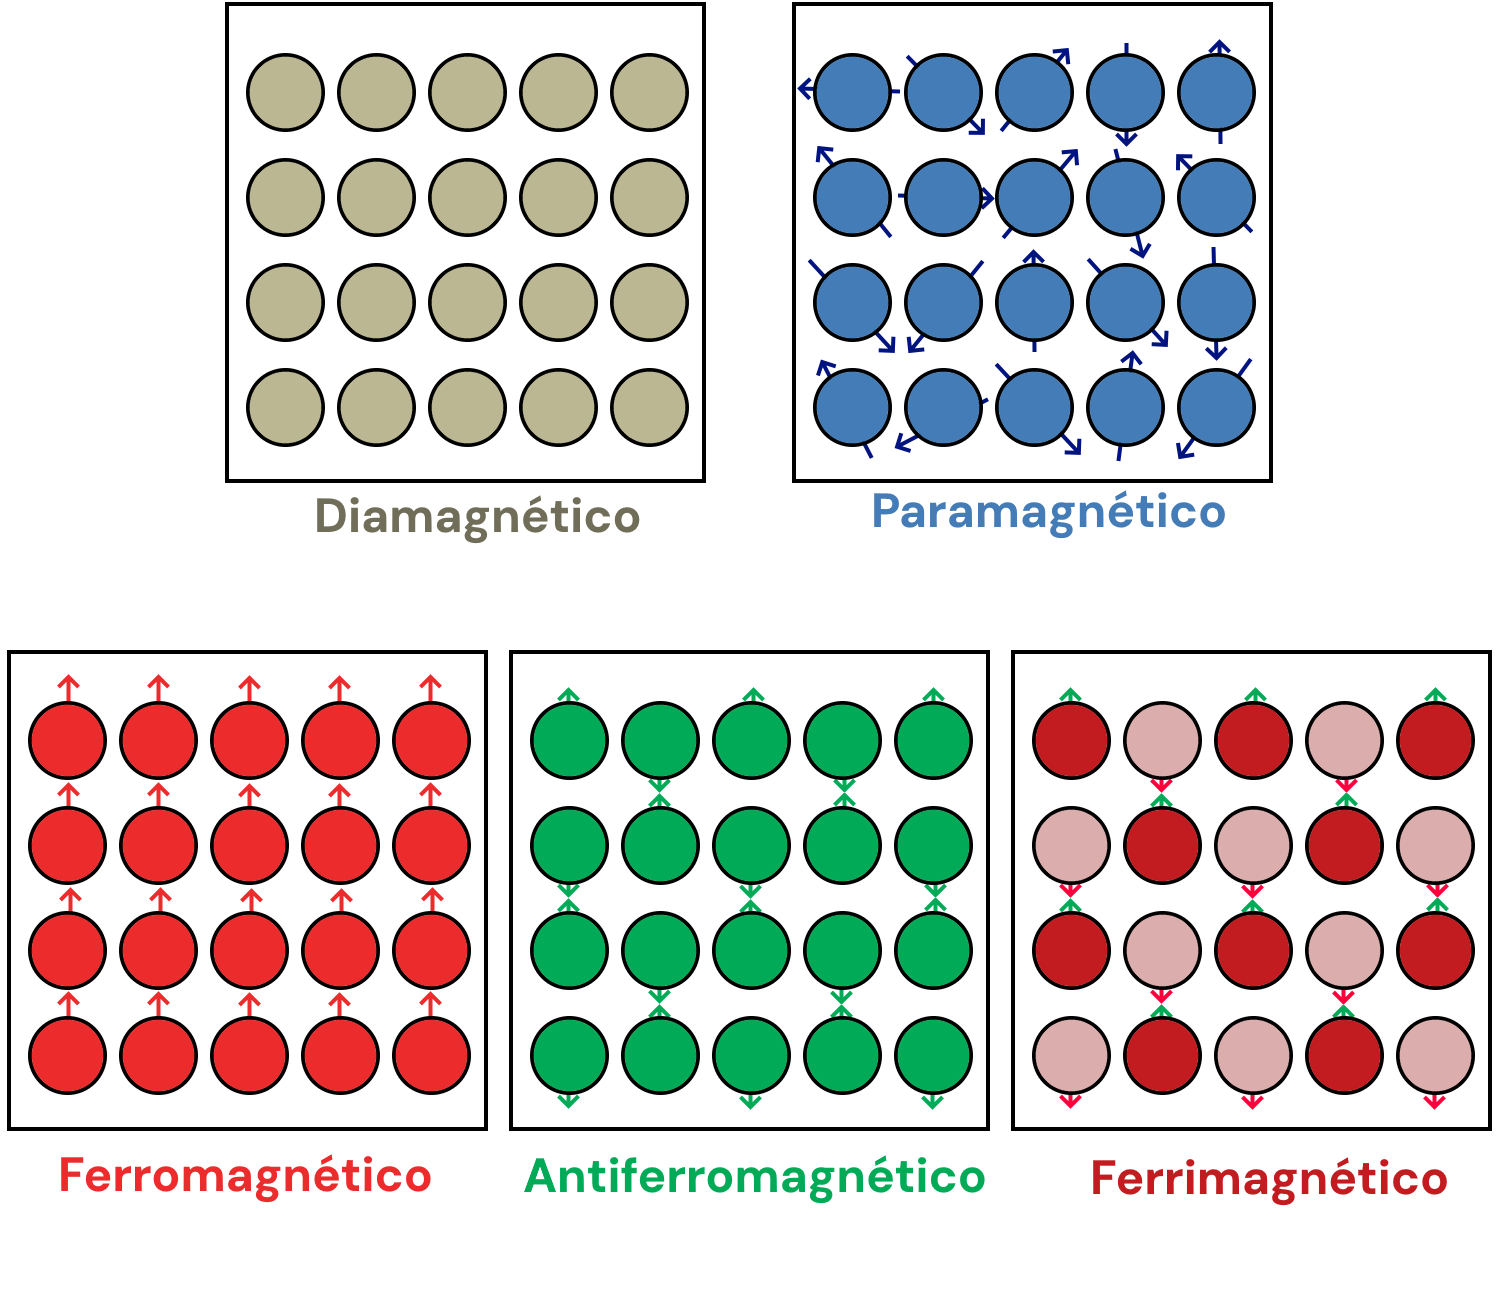
\includegraphics[width=0.7\textwidth]{fig/types.png}
    \caption{Tipos de materiales magnéticos. Adaptado de \cite{Prasad2023}.}
    \label{diagmaterialesmagneticos}
\end{figure}
Clasificando a través de su respuesta a campos externos, podemos dividir los materiales en 5 tipos:
\begin{itemize}
\item \textbf{Diamagnéticos:} (Figura \ref{diagmaterialesmagneticos}a) Cuando un material diamagnético es expuesto a un campo magnético externo, éste presenta una magnetización en el sentido opuesto, es decir, $\chi<0$. Esta magnetización suele ser relativamente débil en comparación con otros fenómenos como el paramagnetismo o el ferromagnetismo \cite{griffiths2023introduction}.
\item \textbf{Paramagnéticos:} (Figura \ref{diagmaterialesmagneticos}b) Cuando un campo magnético ($H$) actúa sobre un material, el momento magnético de cada uno de sus electrones tiende a alinearse de forma paralela o antiparalela al campo. Si todos los electrones están apareados, sus momentos magnéticos se cancelarán entre sí aún después de alinearse, sin embargo esta cancelación no ocurre en aquellos materiales que poseen un electrón desapareado, en este caso, antes de aplicar $H$, los momentos magnéticos individuales en el material apuntan en direcciones aleatorias, dando como resultado una magnetización nula, pero al exponer el material a un campo, estos momentos se alinean, dejando sin cancelar el que proviene del electrón desapareado, dando como resultado una magnetización en el mismo sentido, es decir, $\chi>0$ \cite{griffiths2023introduction}.
\item \textbf{Ferromagnéticos:} (Figura \ref{diagmaterialesmagneticos}c) De forma similar a los materiales paramagnéticos, éstos poseen una susceptibilidad positiva, sin embargo, poseen un orden magnético intrínseco. Dentro de un material ferromagnético existen dominios magnéticos, es decir, zonas del material donde los momentos magnéticos forman una red en la cual apuntan todos en una misma dirección, estas, al ser expuestas a un campo magnético que esté en la misma dirección, comienzan a crecer a expensas de las zonas que apuntan en direcciones distintas, lo cual, macroscópicamente, causa una magnetización positiva, aún si ésta no está relacionada linealmente con el campo externo, como se verá más adelante \cite{coey2010magnetism}.
\item \textbf{Antiferromagnéticos:} (Figura \ref{diagmaterialesmagneticos}d) De manera muy similar a los materiales ferromagnéticos, éstos poseen un orden magnético intrínseco y por lo tanto dominios magnéticos, la diferencia entre ambos tipos de materiales radica en que los antiferromagnéticos poseen además una subred cuyos momentos magnéticos tienen la misma magnitud pero que apunta en sentido opuesto a la otra, por lo cual, aún dentro de un mismo dominio, la magnetización neta es 0 \cite{coey2010magnetism}.
\item \textbf{Ferrimagnéticos:} (Figura \ref{diagmaterialesmagneticos}e) Similares a los materiales antiferromagnéticos, éstos también poseen dominios magnéticos con dos redes de momentos magnéticos, sin embargo, en este caso ambas redes no tienen la misma magnitud, e inclusive pueden tener direcciones distintas, dando como resultado una magnetización diferente de 0, pero que suele ser menor a la de un material ferromagnético \cite{coey2010magnetism}.
\end{itemize}
\subsection{Histéresis}
Se dice que un fenómeno presenta histéresis cuando éste no sólo depende de las condiciones actuales en las que se encuentre, sino también de las condiciones en las que ha estado antes.

Este fenómeno se observa en materiales magnéticos que presentan un orden magnético intrínseco, es decir, materiales ferro, antiferro y ferrimagnéticos.

Éste fenómeno ocurre debido al cambio de tamaño de los dominios magnéticos al aplicarse un campo externo. Retirar el campo no hará que el material regrese a su estado inicial, sino que es necesario aplicar un campo en el sentido opuesto para que ésto ocurra.
\begin{figure}[H]
    \centering
    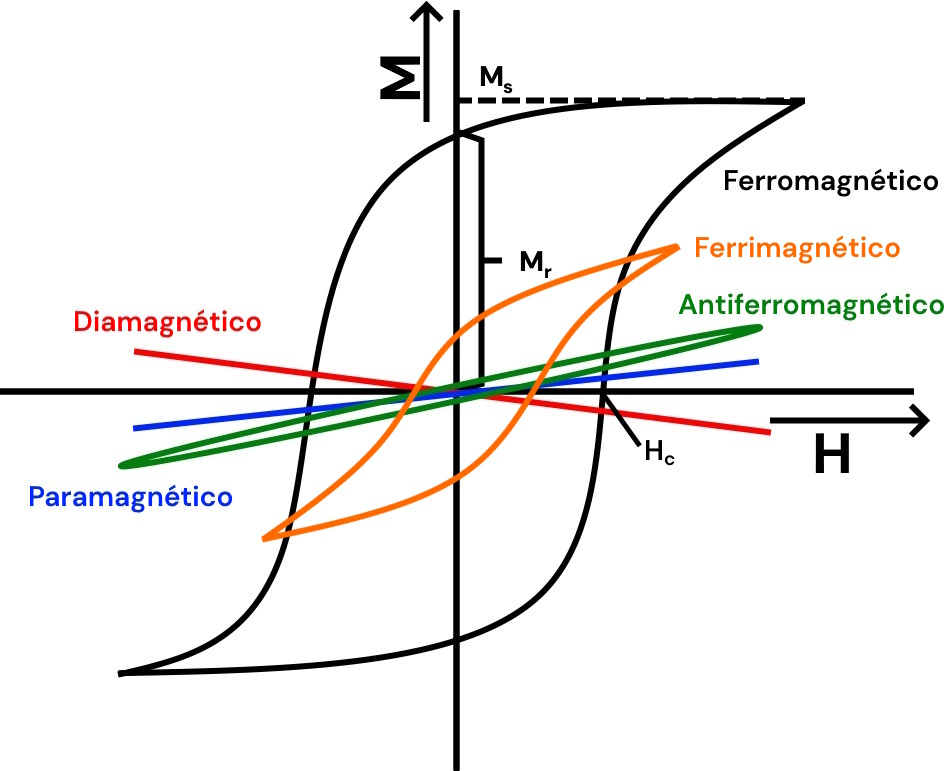
\includegraphics[width=0.55\textwidth]{fig/histeresis1.jpg}
    \caption{Gráfica del comportamiento de la magnetización según el campo externo para los distintos tipos de materiales magnéticos. Adaptado de \cite{Buschow2003}.}
    \label{diaghist}
\end{figure}
Como es posible observar en la Figura \ref{diaghist}, los materiales dia y paramagnéticos no presentan éste comportamiento, su magnetización siempre es la misma para el mismo campo externo. 

Sin embargo, todos los otros materiales presentan un ciclo de histéresis, es decir, su magnetización depende no solo del campo externo, sino también de las condiciones anteriores, cuando el campo externo se retira, no regresan a una magnetización 0, sino que tienen una magnetización remanente, marcada en la figura como $M_r$ para el material ferromagnético. Además, para éstos materiales se puede definir un campo de saturación ($M_s$), éste ocurre cuando el cristal se acerca a contener sólo un dominio magnético, por lo cual su magnetización se acerca asintóticamente a éste valor. Finalmente, $H_c$ se refiere al campo externo necesario para que la magnetización regrese a 0.
\section{Ortoferritas de Tierras Raras}

\subsection{Propiedades Magnéticas}

\subsection{Aplicaciones}
\end{document}